\documentclass[11pt,a4paper]{article}
\usepackage[margin=1in, headheight=14pt]{geometry}
\usepackage{amsfonts,amsmath,amssymb,suetterl}
\usepackage{lmodern}
\usepackage[T1]{fontenc}
\usepackage{fancyhdr}
\usepackage{float}
\usepackage[utf8]{inputenc}
\usepackage{fontawesome}
\usepackage{enumerate}
\usepackage{physics}
\usepackage{tikz}
\usepackage{mathrsfs}
\usepackage[nodisplayskipstretch]{setspace}

\DeclareUnicodeCharacter{2212}{-}

\setstretch{1.5}
\renewcommand{\footrulewidth}{0pt}

\parindent 0ex
\setlength{\parskip}{1em}

\begin{document}
  %
	\begin{singlespace}
		\begin{center}
			\Huge Queen Mary\\
			\LARGE University of London
		\end{center}
		\Large \textbf{MTH5123} \hfill \Large \textbf{Differential Equations,} \hfill \Large \textbf{Autumn 2020}\\
		\large \textbf{Coursework 5 Part 1: week 10 – Selected Solutions} \hfill \large \textbf{W. Huang}
		\rule{\textwidth}{0.4pt}
	\end{singlespace}
	%
	\textbf{I. Practice Problems}\par
	\textbf{A.} Determine the type of equilibrium at $y_1 = 0,\ y_2 = 0$ for the following ODE systems.\par
	A remind of Coursework 8 and the solutions
	\begin{enumerate}[1)]
		\item $\dot{y} = -\frac{1}{2}y_1 + \frac{5}{2}y_2,\ \dot{y_2} = \frac{5}{2}y_1-\frac{1}{2}y_2,\ y_1(0) = a,\ y_2(0) = b$. The solution to this I.V.P. is given by $y_1=\frac{1}{2}(a+b)e^{2t}+\frac{1}{2}(a-b)e^{-3t},\ y_2 = \frac{1}{2}(a+b)e^{2t}-\frac{1}{2}(a-b)e^{-3t}$.
		\item $\dot{y_1} = -y_1+5y_2,\ \dot{y_2} = -y_1+y_2,\ y_1(0) = 0,\ y_2(0) = 4$. The solution to this I.V.P. is given by $y_1 = 10 \sin 2t,\ y_2 = 2 \sin 2t + 4 \cos 2t$.
	\end{enumerate}
	%
	\textbf{Solutions:}\\
	\textbf{(1) The fixed point is a saddle, because we have the two real eigenvalues, one positive and one negative for this linear ODE systems.}\par
	%
	(Revision of Sketching phase portraits: Choosing the initial conditions such that $a = b$ we have $y_1 = y_2 = ae^{2t}$ for any $t$, and this line defines one of the invariant manifolds. Along this line the motion is away from the origin towards $\pm \infty$ for $t \to \infty$ (for $a > 0$ and $a < 0$, respectively). The second invariant manifold $y_2 = -y_1$ corresponds to the initial conditions $b = -a$. Along this line the motion is towards the origin, i.e., for $t \to \infty$ we have $y_2 = -y_1 \to 0$. For initial conditions away from the two invariant manifolds we have asymptotically $y_2\approx y_1\approx \frac{1}{2}(a+b)e^{2t}$ for $t\to \infty$. This means the typical trajectories are hyperbolic-like curves whose tangent is parallel asymptotically to the $y_2 = y_1$ direction for $t \to \infty$ and is parallel to the $y_2 = -y_1$ direction for $t \to -\infty$; see the figure to the end (left).)\par
	%
	\textbf{(2)The fixed point is a centre, because the eigenvalues are two complex numbers with the real part (or TrA) equals to $0$.}\par
	In addition, according to the solution to this IVP, the trajectories must be ellipses; see the figure below for the particular trajectory passing through the given initial conditions.
	%
	\begin{figure}[H]
		\centering
			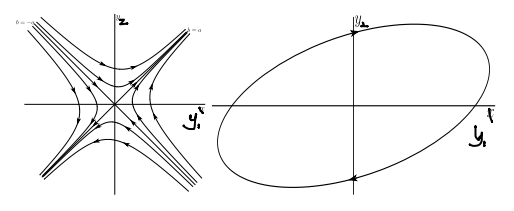
\includegraphics[width=0.75\textwidth]{pdf1201.PNG}
			\caption{Left: The phase portrait for problem $A1$) featuring a saddle. Right: The trajectory solving the initial value problem $A2$). The equilibrium at $(0,0)$ is a center.}
	\end{figure}
	%
	\textbf{B.} Determine the general solution, sketch the phase portraits and determine the type of equilibrium at $y_1 = 0,\ y_2 = 0$ for the following systems of linear differential equations:
	\begin{enumerate}[\bfseries 1)]
		\item $\dot{y_1} = -y_1+6y_2,\ \dot{y_2} = -3y_1 + 8y_2$\\
		\textbf{Solution:} First we rewrite the system in the matrix form $\dot{\vb{y}} = A\vb{u}$, where
		$A
		=
		\begin{pmatrix}
			-1 & 6\\
			-3 & 8
		\end{pmatrix}
		$.
		Next we obtain the characteristic equation and determine the eigenvalues:
		$$
		(-1-\lambda)(8-\lambda)+18
		= \lambda^2-7\lambda + 10
		= 0,\ \lambda_1 = 5\ \lambda_2 = 2
		$$
		Thus, the equilibrium at $(0, 0)$ is an unstable node source, because both eigenvalues are positive. Then we determine the eigenvector components for $\lambda_1 = 5$:
		$$
		\begin{pmatrix}
			-1 & 6\\
			-3 & 8
		\end{pmatrix}
		\begin{pmatrix}
			p_1\\
			q_1
		\end{pmatrix}
		=
		5
		\begin{pmatrix}
			p_1\\
			q_1
		\end{pmatrix}
		\quad
		\Rightarrow
		\quad
		\begin{array}{l}
			-p_1 + 6q_1 = 5p_1\\
			-3p_1 + 8q_1 = 5q_1
		\end{array},
		$$
		which gives $p_1 = q_1$ so that the corresponding eigenvector can be chosen to
		$
		\vb{u_1}
		=
		\begin{pmatrix}
			1\\
			1
		\end{pmatrix}
		$.
		Finally, the general solution to the system of ODEs is given by $\lambda_1 = 2$ is given by 
		$
		\vb{u_2}
		=
		\begin{pmatrix}
			1\\
			1/2
		\end{pmatrix}
		$.
		Finally, the general solution to the system of ODEs is given by
		$$
		\begin{pmatrix}
			y_1\\
			y_2
		\end{pmatrix}
		=
		C_1e^{5t}
		\begin{pmatrix}
			1\\
			1
		\end{pmatrix}
		+ C_2e^{2t}
		\begin{pmatrix}
			1\\
			1/2
		\end{pmatrix}
		$$
		or in components
		$$
		y_1(t) = C_1e^{5t} + C_2e^{2t},\ y_2(t) = c_1e^{5t} + \frac{1}{2}C_2e^{2t}.
		$$
		\begin{figure}[H]
			\centering
				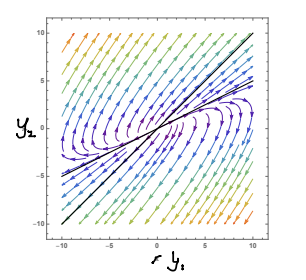
\includegraphics[width=0.55\textwidth]{pdf1202.PNG}
				\caption{The phase portrait for problem ($B1$) featuring an unstable node source.}
		\end{figure}
		\item $\dot{y_1} = -y_1+y_2,\ \dot{y_2}=y_1-y_2$\\
		\textbf{Solution:} We rewrite the system in the matrix form $\vb{\dot{x}} = A\vb{u}$ with
		$
		A
		=
		\begin{pmatrix}
			-1 & 1\\
			1 & -1
		\end{pmatrix}
		$.
		The characteristic equation is $(-1-\lambda)(-1-\lambda)-1=\lambda^2+2\lambda=0,\ \lambda_1 = 0,\ \lambda_2 = -2$. \textbf{Thus, the equilibrium at $(0, 0)$ is stable, as one eigenvalue is negative and the other is zero.} The corresponding eigenvector can be chosen as
		$
		\vb{u_1}
		=
		\begin{pmatrix}
			1\\
			1
		\end{pmatrix}
		$
		and
		$
		\vb{u_2}
		=
		\begin{pmatrix}
			1\\
			-1
		\end{pmatrix}
		$.
		Finally, the general solution to the system of ODEs is given by
		$$
		\begin{pmatrix}
			y_1\\
			y_2
		\end{pmatrix}
		=
		C_1
		\begin{pmatrix}
			1\\
			1
		\end{pmatrix}
		+
		C_2e^{-2t}
		\begin{pmatrix}
			1\\
			-1
		\end{pmatrix}
		$$
		or in components
		$$
		y_1(t) = C_1+C_2e^{-2t},\ y_2(t) = C_1 - C_2e^{-2t}.
		$$
		Note: In the above system, we have two real eigenvalues and one eigenvalue is zero. All points on the line of the eigenvector
		$
		\vb{u_1}
		=
		\begin{pmatrix}
			1\\
			1
		\end{pmatrix}
		$
		obtained under $\lambda = 0$ are all equilibrium points. You can check this by the ODE, when $y_2 = y_1$ both $\dot{y_1} = 0$ and $y_2 = 0$. The equilibrium at $(0, 0)$ is stable (see the phase portraits below) but not a stable node sink.
		\begin{figure}[H]
			\centering
				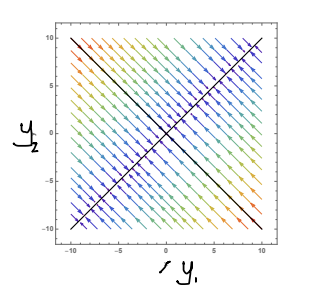
\includegraphics[width=0.55\textwidth]{pdf1203.PNG}
				\caption{The phase portrait for problem B2) featuring a stable equilibrium}
		\end{figure}
		\item $\dot{y_1} = -4y_1-8y_2,\ \dot{y_2} = 4y_1+4y_2$\\
		\textbf{Solution:} We rewrite the system in the matrix form $\vb{\dot{y}} = A\vb{u}$ with
		$
		A
		=
		\begin{pmatrix}
			-4 & -8\\
			4 & 4
		\end{pmatrix}
		$. The characteristic equation is
		$$
		(-4-\lambda)(4-\lambda) + 32
		= \lambda^2 + 16
		= 0
		$$
		which yields two complex-conjugate eigenvalues $\lambda_1 = 4i,\ \lambda_2 = -4i$. \textbf{we can know that the equilibrium at $(0, 0)$ is a center, because the two eigenvalues are complex and their real parts both equal to zero.} The eigenvector components for $\lambda_1 = 4i$ are obtained by
		$$
		\begin{pmatrix}
			-4 & -8\\
			4 & 4
		\end{pmatrix}
		\begin{pmatrix}
			p_1\\
			q_1
		\end{pmatrix}
		=
		4i
		\begin{pmatrix}
			p_1\\
			q_1
		\end{pmatrix}
		\quad
		\Rightarrow
		\quad
		\begin{array}{l}
			-4p_1-8q_1 = 4ip_1\\
			4p_1 + 4q_1 = 4iq_1
		\end{array}.
		$$
		This gives $q_1 = -\frac{1+i}{2}p_1$ so that the corresponding eigenvector can be chosen, for example, as
		$
		\vb{u_1}
		=
		\begin{pmatrix}
			2\\
			-1-i
		\end{pmatrix}
		$. We can immediately conclude that the eigenvector corresponding to
		$\lambda_2 = -4i$ can be chosen in the complex conjugate form
		$
		\vb{u_2}
		=
		\begin{pmatrix}
			2\\
			-1+i
		\end{pmatrix}
		$. Finally, the general solution to the system of ODEs can be written in the from
		$$
		\begin{pmatrix}
			y_1\\
			y_2
		\end{pmatrix}
		= C_1e^{4it}
		\begin{pmatrix}
			2\\
			-1-i
		\end{pmatrix}
		+ C_2e^{-4it}
		\begin{pmatrix}
			2\\
			-1+i
		\end{pmatrix}
		$$
		or in components

		$$
		y_1(t) = 2C_1e^{4it} + 2C_2e^{-4it},\ y_2(t) = (-1-i)C_1e^{4it} + (-1+i)C_2e^{-4it}.
		$$
		For the initial conditions $y_1(0) = a,\ y_2(0) = b$, where $(a, b)$ can be any point in the phase plane
		\begin{equation*}
			\begin{gathered}
				y_1(0)
				= C_1+C_2
				= a/2,\ 
				y_2(0)
				= -1(C_1+C_2) + (C_2-C_1)i
				= b\\
				\Rightarrow\ 
				C_1 = \frac{a}{4}+\frac{2b+a}{4}i,\ 
				C_2 = \frac{a}{4}-\frac{2b+a}{4}i,
			\end{gathered}
		\end{equation*}
		Thus the solution to this IVP will be
		\begin{equation*}
			\begin{gathered}
				y_1(t) = 2(\frac{a}{4}+\frac{2b+a}{4}i)e^{4it} + 2(\frac{a}{4}-\frac{2b+a}{4}i)e^{-4it}
				= a\cos 4t - (2b+a)\sin 4t,\\
				y_2(t) = (-1-i)(\frac{a}{4}+\frac{2b+a}{4})e^{4it}+(-1+i)(\frac{a}{4}-\frac{2b+a}{4}i)e^{-4it}
				= (b+a)\sin 4t+b\cos 4t.
			\end{gathered}
		\end{equation*}
		As the phase portrait is a centre. If we plot one ellipse (one trajectory), then all other trajectories are just a set of nested ellipses around the equilibrium point in this linear system $(0, 0)$. Thus, pick any values for $(a, b)$, e.g. $(1, 0)$, the solution to this IVP becomes
		\begin{equation*}
			\begin{gathered}
				y_1(t) = \cos 4t - \sin 4t,\\
				y_2(t) = \sin 4t.
			\end{gathered}
		\end{equation*}
		You can plot the ellipse by chose $t = 0,\ \frac{\pi}{16},\ \frac{2\pi}{16},\ \frac{4\pi}{16},\ \frac{5\pi}{16},\ \frac{6\pi}{16},\ \ldots$, which is the black ellipse in the Figure \ref{f4}. Then you draw rest trajectories accordingly.
		%
		\begin{figure}[H]
			\centering
				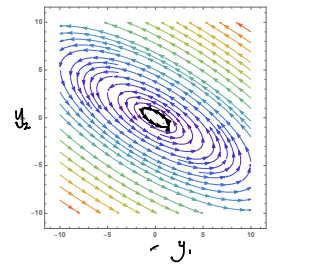
\includegraphics[width=0.55\textwidth]{pdf1204.PNG}
				\caption{ The phase portrait for problem B3) featuring a center.}
				\label{f4}
		\end{figure}
		If you transform the $y_1y_2$ coordinates to new coordinates as described in our lecture, the trajectories will becomes counterclockwise circles around $(0, 0)$.
	\end{enumerate}
	%
	\textbf{C.} Determine the type of fixed point for the dynamical systems
	$$
	\dot{y_1} = 4y_2,\ \dot{y_2} = -y_1.
	$$
	Then determine the solutions of the corresponding initial value problems for the general initial conditions $y_1(0) = a,\ y_2(0) = b$. Finally sketch the phase portraits in the $(y1, y2)$ phase plane.\par
	\text{Solution.} The matrix associated with this system is given by
	$
	A
	=
	\begin{pmatrix}
		0 & 4\\
		-1 & 0
	\end{pmatrix}
	$.
	The characteristic equation is $\lambda^2 +4 = 0$ with two complex conjugate roots $\lambda_1 = 2i,\ \lambda_2 = -2i$.\\
	\textbf{As the eigenvalues are complex conjugate and their real parts equal to zero, the corresponding fixed point is a center.}\\
	The eigenvector corresponding to $\lambda_1 = 2i$ can be found from
	$$
	\begin{pmatrix}
		0 & 4\\
		-1 & 0
	\end{pmatrix}
	\begin{pmatrix}
		p_1\\
		q_1
	\end{pmatrix}
	=
	2i
	\begin{pmatrix}
		p_1\\
		q_1
	\end{pmatrix},\quad
	\Rightarrow
	q_1
	=
	\frac{i}{2}p_1
	$$
	so that the eigenvectors are
	$
	\vb{u_1}
	=
	\begin{pmatrix}
		1\\
		\frac{i}{2}
	\end{pmatrix}
	$
	and
	$
	\vb{u_2}
	=
	\begin{pmatrix}
		1\\
		-\frac{i}{2}
	\end{pmatrix}
	$.
	The general solution has the form
	$$
	\begin{pmatrix}
		y_1\\
		y_2
	\end{pmatrix}
	= C_1e^{2it}
	\begin{pmatrix}
		1\\
		\frac{i}{2}
	\end{pmatrix}
	+ C_2e^{-2it}
	\begin{pmatrix}
		1\\
		-\frac{i}{2}
	\end{pmatrix}.
	$$
	The initial conditions yield
	$$
	y_1(0) = C_1 + C_2 = a,\ y_2(0) = \frac{i}{2}(C_1-C_2)=b\ \Rightarrow\ C_1 = \frac{1}{2}(a-2bi),\ C_2 = \frac{1}{2}(a+2bi)
	$$
	so that the solution to the general initial value problem is given by
	$$
	y_1 = \frac{1}{2}(a-2ib)e^{2it} + \frac{1}{2}(a+2ib)e^{-2it} = a\cos 2t+2b\sin 2t,
	$$
	and similarly
	$$
	y_2 = \frac{i}{4}(a-2ib)e^{2it} - \frac{1}{4}(a+2ib)e^{-2it} = -\frac{a}{2}\sin 2t + b\cos 2t.
	$$
	We notice that $y_1^2 + 4y_2^2 = a^2 + 4b^2$ describing ellipses in phase space. The check the direction of the trajectories (arrows), we can pick up any initial point, for example,describing ellipses in phase space. The check the direction of the trajectories (arrows), we can pick up any initial point, for example, $y_1(0) = 1,\ y_2(0) = 0$, then the tangent vector at this point is
	$
	\begin{pmatrix}
		\dot{y_1}(0)\\
		\dot{y_2}(0)
	\end{pmatrix}
	=A
	\begin{pmatrix}
		y_1(0)\\
		y_2(0)
	\end{pmatrix}
	=
	\begin{pmatrix}
		0 & 4\\
		-1 & 0
	\end{pmatrix}
	\begin{pmatrix}
		1\\
		0
	\end{pmatrix}
	=
	\begin{pmatrix}
		0\\
		-1
	\end{pmatrix}
	$.
	Thus the trajectory starting at $(1, 0)$ will move towards negative $y$ values (clockwise).\\
	\textbf{Note the trajectories here are clockwise as it is in the original $y_1y_2$ coordinates. If you transform the $y_1y_2$ coordinates to new coordinates as described in our lecture, the trajectories will becomes counterclockwise circles around $(0, 0)$.}
	%
	\begin{figure}[H]
		\centering
			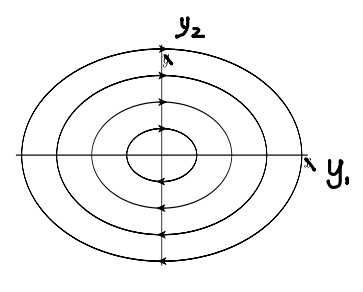
\includegraphics[width=0.55\textwidth]{pdf1205.PNG}
			\caption{Phase portrait for problem C featuring a centre.}
	\end{figure}
	%
	\textbf{D.} Determine the solution of the initial value problem
	$$
	\dot{y_1} = y_1-4y_2,\ \dot{y_2} = 4y_1+y_2,\ y_1(0) = 0,\ y_2(0) = 1,\ t \geq 0
	$$
	and the type of fixed point. Then sketch the trajectory in the $(y_1, y_2)$ phase plane corresponding to the chosen initial values in the specified range of $t$\par
	\textbf{Solution.} The matrix associated with the system is given by
	$
	A
	=
	\begin{pmatrix}
		1 & -4\\
		4 & 1
	\end{pmatrix}
	$
	The characteristic equation is $\lambda^2 - 2\lambda +17=0$ with two complex conjugate roots $\lambda_1 = 1+4i,\ \lambda_2 = 1-4i$. The eigenvector corresponding to $\lambda_1 = 1+4i$ can be found from
	$$
	\begin{pmatrix}
		1 & -4\\
		4 & 1
	\end{pmatrix}
	\begin{pmatrix}
		p_1\\
		q_1
	\end{pmatrix}
	=
	(1+4i)
	\begin{pmatrix}
		p_1\\
		q_1
	\end{pmatrix}\quad
	\Rightarrow
	q_1 = -ip_1
	$$
	so that the eigenvectors are
	$
	\vb{u_1}
	=
	\begin{pmatrix}
		1\\
		-i
	\end{pmatrix}
	$
	and
	$
	\vb{u_2}
	=
	\begin{pmatrix}
		1\\
		i
	\end{pmatrix}
	$.
	The general solution has the form
	$$
	\begin{pmatrix}
		y_1\\
		y_2
	\end{pmatrix}
	=
	C_1e^{t+4it}
	\begin{pmatrix}
		1\\
		-i
	\end{pmatrix}
	+ C_2e^{t-4it}
	\begin{pmatrix}
		1\\
		i
	\end{pmatrix}.
	$$
	The initial conditions yield
	$$
	y_1(0) = C_1+C_2 = 0,\ y_2(0) = C_1(-i)+C_2i = 1,\ \Rightarrow\ C_1 = \frac{i}{2},\ C_2 = \frac{-i}{2}
	$$
	so that the solution to the general initial value problem is given by
	$$
	y_1 = \frac{i}{2}e^{t+4it} - \frac{i}{2}e^{t-4it} = -e^t\sin 4t.
	$$
	and similarly
	$$
	y_2 = \frac{i}{2}(-i)e^{t+4it} - \frac{i}{2}ie^{t-4it} = e^t\cos 4t.
	$$
	The fixed point is an unstable focus and trajectories are spiraling away from the origin for $t \to \infty$ For the specified initial conditions the initial tangent vector to the trajectory is $\dot{y_1}(0) = -4,\ \dot{y_2} = 1$ so that the rotation goes anticlockwise; see the sketch below.
	%
	\textbf{III. Applications involving Dynamical Systems}\par
	\textbf{A.} Using the relation between charge and current given by $I = dQ/dt$, rewrite the following
	$$
	L\frac{dI}{dt} + RI + \frac{1}{C}Q = E(t)
	$$
	as a second order equation in the charge Q. Use this to obtain an ODE for the current $I$ as
	$$
	L\frac{d^2I}{dt^2} + R\frac{dI}{dt} + \frac{1}{C}I = \dot{E}(t).
	$$
	%
	\begin{figure}[H]
		\centering
			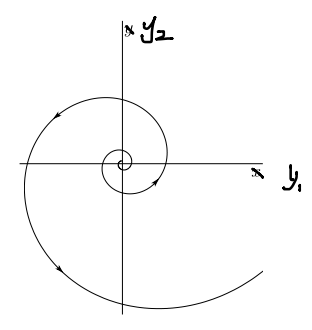
\includegraphics[width=0.35\textwidth]{pdf1206.PNG}
			\caption{The trajectory solving this initial value problem) with an unstable focus.}
	\end{figure}
	%
	\textbf{Solution.} Let differentiation with respect to t be denoted by a dot (Newton’s notation for independent variable as time t). Then we have $I = \dot{Q}$ and consequently, $\dot{I} = \ddot{Q}$.  The given equation can be rewritten in terms of $Q$ as
	$$
	E(t) = L\frac{dI}{dt} + RI + \frac{1}{C}Q = L\dot{I} + RI + \frac{1}{C}Q = L\ddot{Q}+R\dot{Q} + \frac{1}{C}Q,
	$$
	which is a second-order equation in $Q.$\\
	We can either differentiating this 2nd-order ODE or the original 1st-order ODE over $t$, and using the fact that $\dot{Q} = I$, we obtain
	$$
	L\dddot{Q}+R\ddot{Q}+\frac{1}{C}\dot{Q} = L\ddot{I} + R\dot{I} + \frac{1}{C}I = \dot{E}(t),
	$$
	which is a second order equation in $I.$\par
	\textbf{B.} Assuming the system is closed and $\dot{E}(t) = 0$, write the second order equation in $I$ as a system of two first order equations using $y_1 = I$ and $y = dI/dt$. Show that $y_1 = 0,\ y_2 = 0$ is a critical point.\par
	\textbf{Solution.} Given $\dot{E}(t) = 0$, we have $L\dot{I}+R\dot{I} + \frac{1}{C}I = 0$. Following the suggested definitions for $x$ and $y$,
	\begin{equation*}
		\begin{aligned}
			&y_1 = I\quad \Rightarrow \quad \dot{y_1} = \dot{I} = y_2\\
			&y_2 = \dot{I} \quad \Rightarrow \quad \dot{y_2} = \ddot{I} = \frac{1}{L}\left(-R\dot{I}-\frac{1}{C}I\right) = \frac{1}{L}\left(-Ry - \frac{1}{C}x\right).
		\end{aligned}
	\end{equation*}
	Rewriting the equation as a linear system, we find
	$$
	\begin{pmatrix}
		\dot{y_1}\\
		\dot{y_2}
	\end{pmatrix}
	=
	\begin{pmatrix}
		0 & 1\\
		-\frac{1}{LC} & -\frac{R}{L}
	\end{pmatrix}
	\begin{pmatrix}
		y_1\\
		y_2
	\end{pmatrix}.
	$$
	We immediately see that $(x, y) = (0, 0)$ is a critical point of the system since both the left and right hand sides vanish for this solution.
\end{document}